\RequirePackage{ifpdf}
\ifpdf
	\documentclass[11pt,oneside,a4paper,pdftex]{article}   %two-page printing
\else
	\documentclass[11pt,twoside,a4paper,dvips]{article}   %two-page printing
\fi

%\documentclass[a4paper, 12pt]{article}
\addtolength{\hoffset}{-1.9cm}
\addtolength{\voffset}{-1.9cm}
\addtolength{\textwidth}{+3.8cm}
\addtolength{\textheight}{+3.8cm}
\usepackage[latin1,utf8]{inputenc}
\usepackage[czech]{babel}
\usepackage{icomma} % ceska desetinna carka
\usepackage{csquotes}
\usepackage{listings}
\usepackage{amsmath}
\usepackage{amsthm}
\usepackage{amsfonts}
\usepackage{mathrsfs}
%\usepackage[T1]{fontenc}
\ifpdf
	\usepackage[pdftex]{graphicx} % dvips or pdftex
\else
	\usepackage[dvips]{graphicx} % dvips or pdftex
\fi
\usepackage[center]{subfigure}
\usepackage{amsfonts}
\usepackage[dvips]{color}               %for using colors
%\usepackage{showframe}                 %zobrazuje okraje stranky
\usepackage[justification=justified,hang]{caption}
\usepackage{textpos}
\usepackage{url}
%\usepackage{fancybox}
\usepackage{verbatim}
\usepackage{fj}
\ifpdf
	\usepackage[pdftex,unicode,colorlinks]{hyperref}
\else
	\usepackage[unicode]{hyperref}
\fi


%FIXME: odlišit font, aby části kódu byly odlišitelné od okolního textu
\lstset{ %
language=Matlab,           % choose the language of the code
basicstyle=\ttfamily,   % the size of the fonts that are used for the code
numbers=none,             % where to put the line-numbers (none, left, ..)
numberstyle=\scriptsize,  % size of the fonts used for the line-numbers
stepnumber=1,             % step between two line-nums. If "1" each line nmbrd
numbersep=10pt,            % how far the line-numbers are from the code
%backgroundcolor=\color{white},
	% choose the background color. You must add \usepackage{color}
showspaces=false,         % show spaces adding particular underscores
showstringspaces=false,   % underline spaces within strings
showtabs=false,           % show tabs within strings
frame=none,	          % adds a frame around the code (single, none, ...)
tabsize=2,	          % sets default tabsize to 2 spaces
captionpos=b,             % sets the caption-position to bottom
breaklines=false,          % sets automatic line breaking
breakatwhitespace=true,   % sets if automatic breaks should only happen at \s
%escapeinside={\%*}{*)}   % if you want to add a comment within your code
}

\title{1. Zpráva pro předmět 3D Počítačové vidění -- A4M33TDV}
\date{29. 11. 2011}
\author{Filip Jareš, jaresfil@fel.cvut.cz}

\begin{document}

\maketitle

\section{Úvod}

Tato zpráva popisuje semestrální práci pro předmět 3D počítačové vidění, jejímž cílem je na základě
dvanácti fotografií vybraného objektu (portálu/dveří) zrekonstruovat nasnímanou scénu a vytvořit
trojrozměrný digitální model této scény.

Práce ještě není dokončená, proto v této verzi zpráva popisuje pouze dosud hotovou část řešení:
výběr scény, zvolenou konfiguraci kamer, nástroj použitý pro odstranění radiálního zkreslení
a~metodu kalibrace kamery. Nakonec potom hledání řídkých korespondencí mezi obrazy a~odhad
epipolární geometrie mezi dvojicemi snímků.

\section{Řešení}

\subsection{Struktura řešení}

Použité řešení úlohy rekonstrukce 3D scény z několika fotografií lze rozdělit na tři hlavní fáze:
(i) zachycení scény a přípravu snímků pro pozdější zpracování; (ii) rekonstrukci řídkého mraku
prostorových bodů z~těchto snímků a (iii) rekonstrukci hustého mraku bodů s použitím stereo párování,
které poskytne husté korespondence mezi dvojicemi obrazů se známou epipolární geometrií.
Tato první verze zprávy popisuje pouze fázi první a částečně fázi druhou.

Důležitým krokem fáze (i) je odstranění radiálního zkreslení. Hlavními částmi fáze (ii) je nalezení
řídkých korespondencí mezi obrazy a použití těchto korespondencí k odhadu epipolární geometrie
dvojic snímků a tedy odhadu relativních rotací a translací dvojic kamer. Následuje \uv{slepování}
takových dvojic kamer, tedy jejich umístění do společného souřadného systému.

V následující části jsou jednotlivé kroky prvních dvou fází (kromě slepování kamer) popsány
podrobněji.

\subsection{Popis řešení}

\subsubsection{Výběr scény}
Jako objekt pro rekonstrukci byly vybrány domovní dveře domu v pražské Jeseniově ulici. Byly
vyfotografovány z dvanácti míst tak, jak je to přibližně znázorněno na \figref{fig:usporadaniKamer}.
Kolmá vzdálenost od dveří byla u všech kamer přibližně stejná (zhruba 4\,m) a dveře byly ze čtyř
míst vyfotografovány vždy ze tří rúzných výškových úrovní (zhruba z výšky 30\,cm, 130\,cm a
200\,cm).
	\begin{figure}[htb]
		\centering
		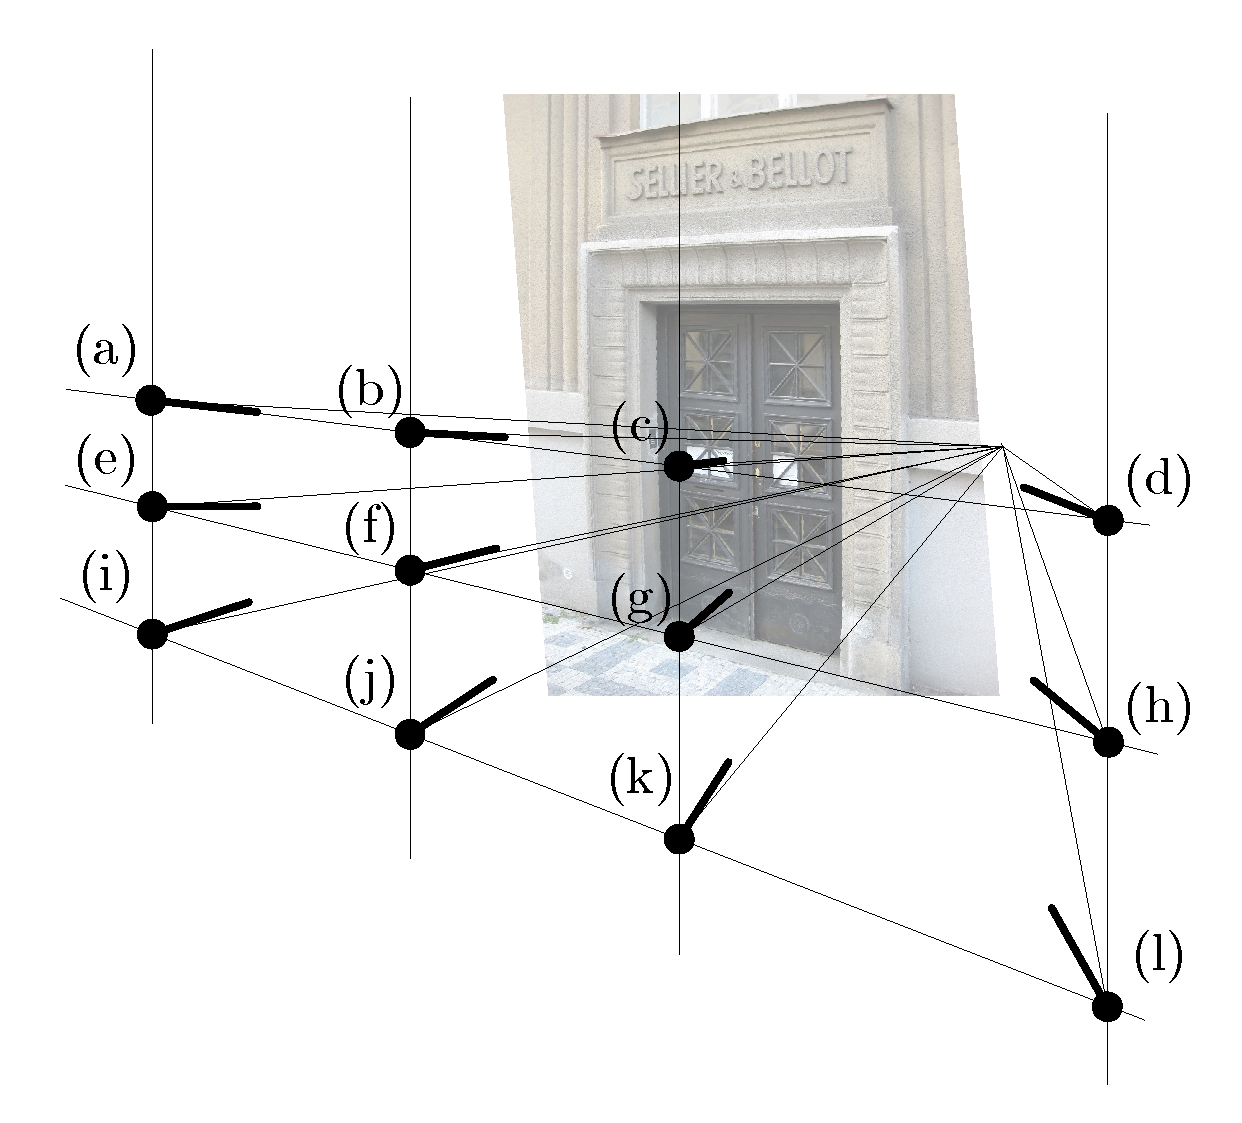
\includegraphics[width=8cm]{pictures/usporadani_kamer.pdf}
		\caption{Schéma uspořádání kamer při snímání scény}
		\label{fig:usporadaniKamer}
	\end{figure}
Fotografie s rozlišením $3264\times2448$ pixelů byly pořízeny fotoaparátem Canon Ixus 80
IS na nejkratší ohniskovou vzdálenost. Zachyceny jsou na \figref{fig:fotografie}.
	\begin{figure}[htbp]
		% dummy content, to make the rendering faster while under construction
			% \centering
			% \subfigure[] {
			% 	\fbox{\begin{minipage}{3cm}\hfill\vspace{4cm}\end{minipage}}
			% 	\label{fig:firstInputImage}
			% }
			% \subfigure[] {
			% 	\fbox{\begin{minipage}{3cm}\hfill\vspace{4cm}\end{minipage}}
			% }
			% \subfigure[] {
			% 	\fbox{\begin{minipage}{3cm}\hfill\vspace{4cm}\end{minipage}}
			% }
			% \subfigure[] {
			% 	\fbox{\begin{minipage}{3cm}\hfill\vspace{4cm}\end{minipage}}
			% }
			% \\
			% \subfigure[] {
			% 	\fbox{\begin{minipage}{3cm}\hfill\vspace{4cm}\end{minipage}}
			% }
			% \subfigure[] {
			% 	\fbox{\begin{minipage}{3cm}\hfill\vspace{4cm}\end{minipage}}
			% 	\label{fig:i0}
			% }
			% \subfigure[] {
			% 	\fbox{\begin{minipage}{3cm}\hfill\vspace{4cm}\end{minipage}}
			% 	\label{fig:i1}
			% }
			% \subfigure[] {
			% 	\fbox{\begin{minipage}{3cm}\hfill\vspace{4cm}\end{minipage}}
			% }
			% \\
			% \subfigure[] {
			% 	\fbox{\begin{minipage}{3cm}\hfill\vspace{4cm}\end{minipage}}
			% }
			% \subfigure[] {
			% 	\fbox{\begin{minipage}{3cm}\hfill\vspace{4cm}\end{minipage}}
			% }
			% \subfigure[] {
			% 	\fbox{\begin{minipage}{3cm}\hfill\vspace{4cm}\end{minipage}}
			% }
			% \subfigure[] {
			% 	\fbox{\begin{minipage}{3cm}\hfill\vspace{4cm}\end{minipage}}
			% }
		% Real pictures:
			\centering
			\subfigure[] {
				\fbox{\includegraphics[width=4.3cm,angle=-90]{pictures/IMG_5959.JPG}}
			      \label{fig:firstInputImage}
			}
			\subfigure[] {
				\fbox{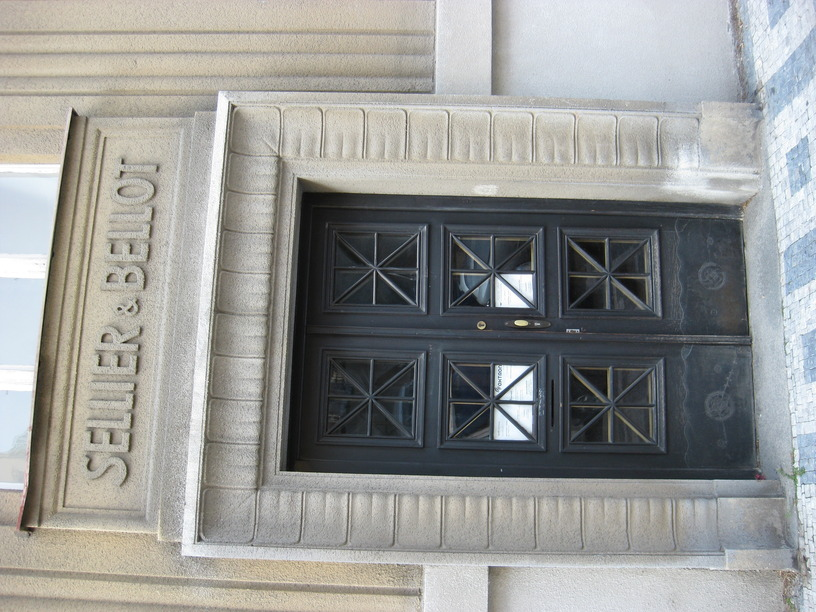
\includegraphics[width=4.3cm,angle=-90]{pictures/IMG_5955.JPG}}
			}
			\subfigure[] {
				\fbox{\includegraphics[width=4.3cm,angle=-90]{pictures/IMG_5962.JPG}}
			}
			\subfigure[] {
				\fbox{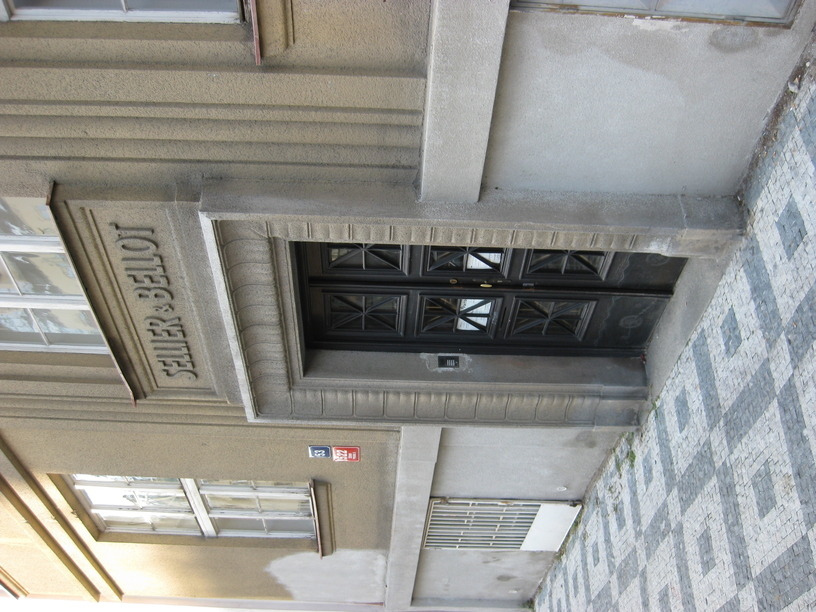
\includegraphics[width=4.3cm,angle=-90]{pictures/IMG_5965.JPG}}
			}
			\\
			\subfigure[] {
				\fbox{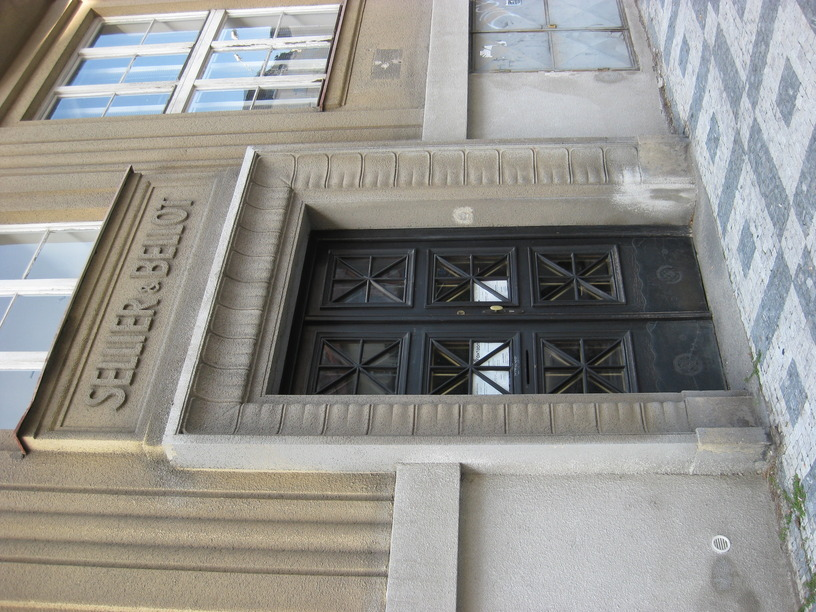
\includegraphics[width=4.3cm,angle=-90]{pictures/IMG_5957.JPG}}
			}
			\subfigure[] {
				\fbox{\includegraphics[width=4.3cm,angle=-90]{pictures/IMG_5954.JPG}}
			      \label{fig:i0}
			}
			\subfigure[] {
				\fbox{\includegraphics[width=4.3cm,angle=-90]{pictures/IMG_5961.JPG}}
			      \label{fig:i1}
			}
			\subfigure[] {
				\fbox{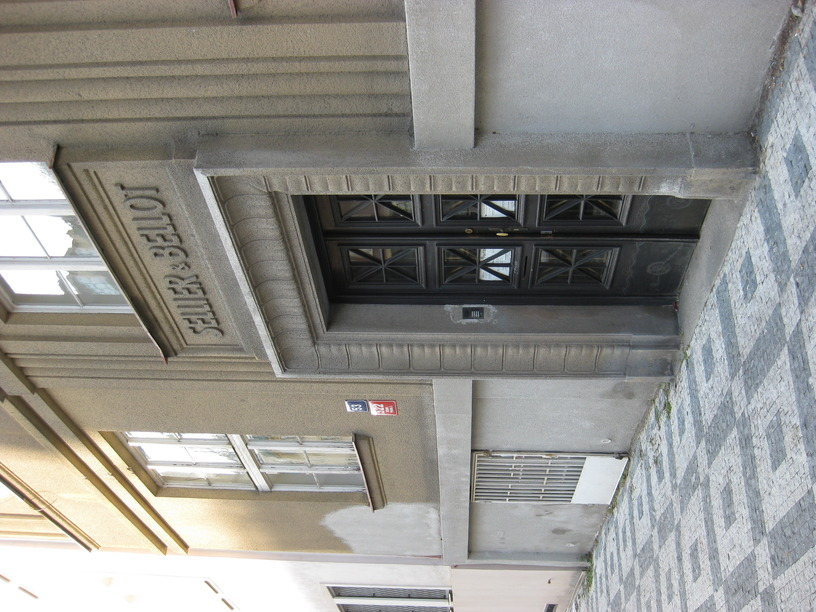
\includegraphics[width=4.3cm,angle=-90]{pictures/IMG_5964.JPG}}
			}
			\\
			\subfigure[] {
				\fbox{\includegraphics[width=4.3cm,angle=-90]{pictures/IMG_5956.JPG}}
			}
			\subfigure[] {
				\fbox{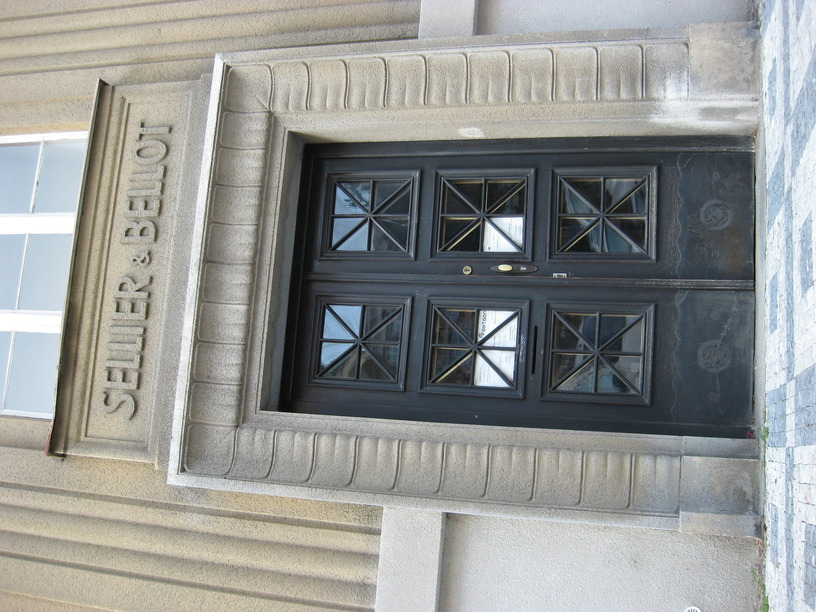
\includegraphics[width=4.3cm,angle=-90]{pictures/IMG_5953.JPG}}
			}
			\subfigure[] {
				\fbox{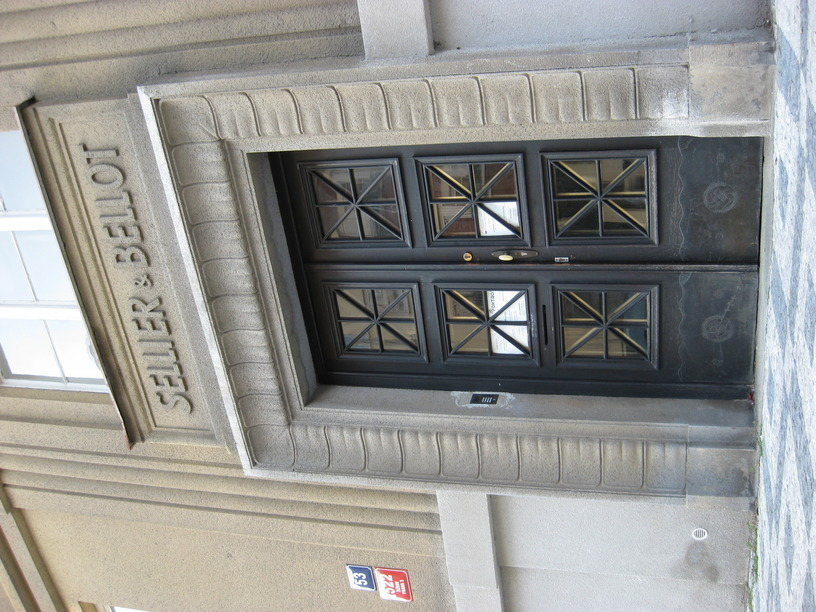
\includegraphics[width=4.3cm,angle=-90]{pictures/IMG_5960.JPG}}
			}
			\subfigure[] {
				\fbox{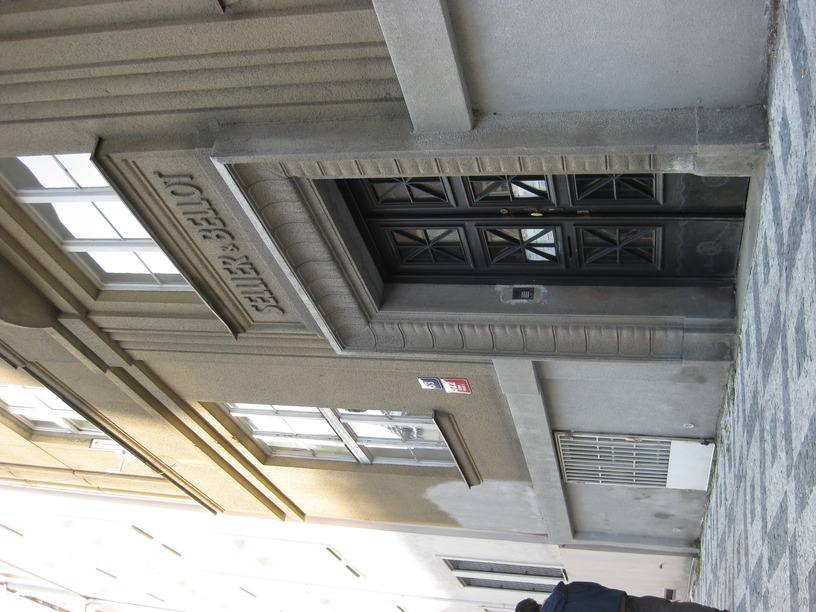
\includegraphics[width=4.3cm,angle=-90]{pictures/IMG_5963.JPG}}
			}
		\caption{Snímky scény, které byly použity pro rekonstrukci, označení obrázků
			odpovídá označení kamer na obrázku \ref{fig:usporadaniKamer}}
		\label{fig:fotografie}
	\end{figure}

\subsubsection{Odstranění radiálního zkreslení a kalibrace kamery} Protože použité algoritmy pra\-cují
s~lineárním modelem kamery, bylo nutné před dalším použitím nafocených snímků nej\-prve odstranit
radiální zkreslení. K tomuto účelu byl použit nástroj \emph{rd\_undistort}, který byl k dispozici od
vyučujících \cite{code_repo}.\footnote{Jak citovat tyto nástroje?} Jako podklad pro kalibraci tohoto
nástroje posloužily tři snímky kalibračního obrazce. Jeden z nich je na obrázku~\ref{fig:radialCalibration}.
% \url{http://cmp.felk.cvut.cz/cmp/courses/TDV/code/rd\_undistort\_20110112.zip}

\def\IAC{\boldsymbol \omega}

K rekonstrukci scény je rovněž potřebná znalost kalibrační matice $\matrix K$ použité kamery
\cite[sekce 8.8]{Hartley2004}.  $\matrix K$ má obecně pět stupňů volnosti.  U fotoaparátu jsme
předpokládali čtver\-co\-vé pixely (bez zkosení), zbylé tři stupně volnosti kalibrační matice jsme
určili na základě znalosti úběžníků třech kolmých směrů v jediném obraze (viz. \figref{fig:kalibraceKamery}).
Z každého páru ta\-ko\-vých ú\-běž\-ní\-ků $\vector u_i$, $\vector u_j$ vyplývá jedna podmínka na obraz
absolutní kuželosečky $\IAC$:
	\begin{equation}
		\vector u_i\T \IAC \vector u_j = 0, \qquad i, j \in \{1, 2, 3\},\quad i \ne j.
	\end{equation}
Kalibrační matici jsme určili z obrazu absolutní kuželosečky na základě vztahu
	\begin{equation} \IAC = (\matrix K \matrix K\T)^{-1} \end{equation}
pomocí Choleskyho faktorizace. Výsledná kalibrační matice byla:
	\begin{equation} \label{eq:matrixK}
		\matrix K = \begin{pmatrix}
				3442,3	& 0		& 1614,3 \\
				0	& 3442,3	& 1185,7 \\
				0	& 0		& 1
			\end{pmatrix}.
	\end{equation}
	\begin{figure}[htb]
		\centering
		\subfigure[] {
			\fbox{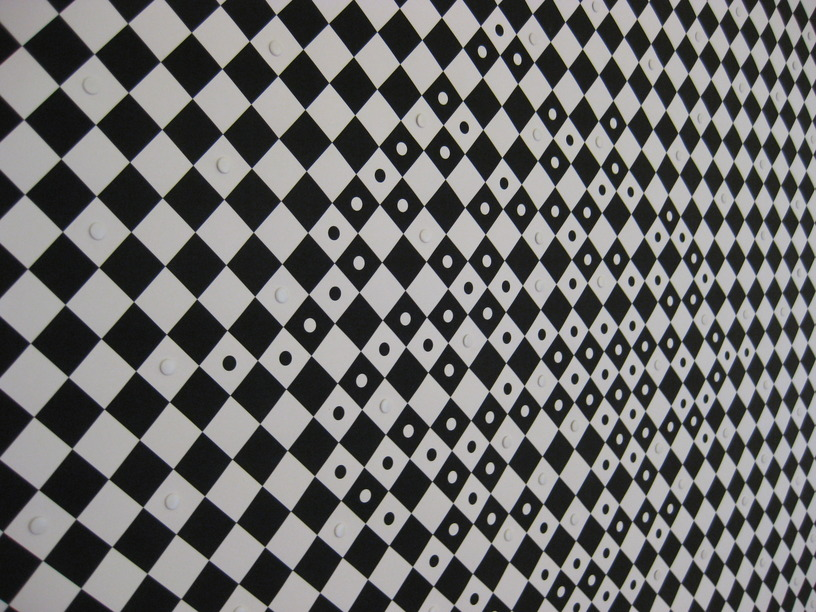
\includegraphics[width=7cm]{pictures/radial_calibration_pattern.jpg}}
			\label{fig:radialCalibration}
		}
		\subfigure[] {
			\fbox{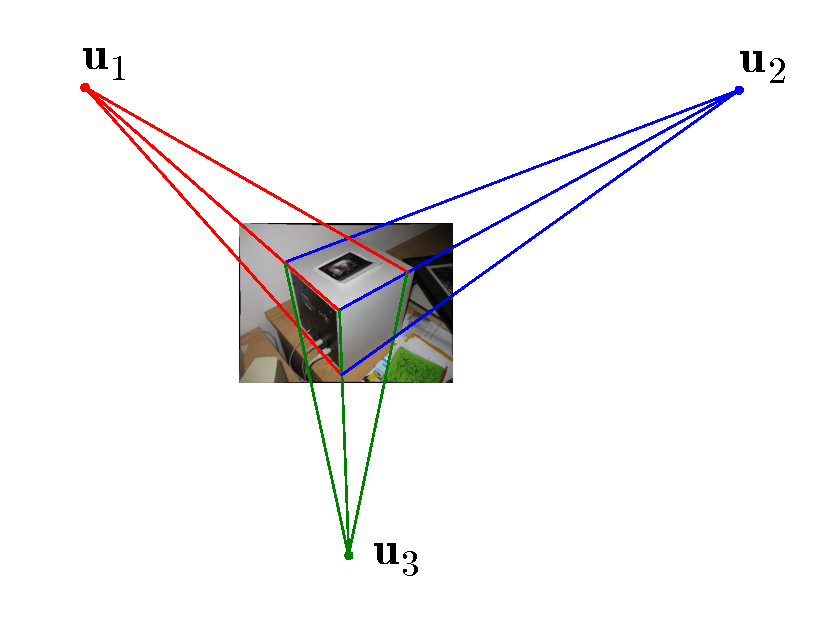
\includegraphics[width=7cm]{pictures/ubezniky_cube.pdf}}
			\label{fig:kalibraceKamery}
		}
		\caption{Snímky použité pro kalibraci: \subref{fig:radialCalibration} vzor použitý
			pro kalibraci nástroje pro odstranění radiálního zkreslení.
			\subref{fig:kalibraceKamery} Snímek kvádru použitého pro
			kalibraci kamery; červeně, zeleně a modře jsou vyznačeny rovnoběžky ve třech
			navzájem kolmých směrech protínající se v jednotlivých úběžnících.}
	\end{figure}

\subsubsection{Nalezení předběžných korespondencí} Pro nalezení řídkých korespondencí mezi body ve
dvojicích obrazů byl opět použit dodaný kód -- \emph{WBS Matcher} \cite{code_repo},
\cite{WBS_Matcher}.  Nejprve byly (pro každý obrázek nezávisle) k automaticky vybraným
\uv{význačným} bodům vypočteny a přiřazeny deskriptory. Na základě porovnání těchto deskriptorů byly
potom vytvořeny korespondence mezi obrazy.

Pro každý snímek vytvořil WBS Matcher přibližně 30\,000 deskriptorů. Počet nalezených předběžných
korespondencí pro pár obrazů se pohyboval mezi 400 až 7\,000. Tyto korespondence byly poté v
následujícím kroku použity pro odhad epipolární geometrie pří\-slu\-šných kamer.


\subsubsection{Odhad epipolární geometrie} Odhad esenciální matice $\matrix E$ daného páru
ka\-mer je založen na použití předběžných korespondencí získaných v~předchozím
kroku. Protože jsou nalezené korespondence kontaminovány chybami, byl jakožto metoda robustního
odhadu použit algoritmus RANSAC \cite{RansacOverview}. Ten je tvořen smyčkou, v níž jsou
opakovaně vytvářeny hypotézy (matice $\matrix E$), pro které je ověřována jejich konzistence
s daty. RANSAC vybere z prověřených hypotéz tu, která je v největší míře kon\-zis\-ten\-tní s daty.

% \paragraph{Def.: Podmínka chirality} \emph{Pár kanonických kamer $\matrix P_1$, $\matrix P_2$ a prostorový
% bod $\vector X$ splňuje podmínku chirality právě tehdy, pokud bod $\vector X$ leží před oběma
% kamerami.}

\paragraph{Vytváření Hypotéz} Esenciální matice, představující hypotézy pro daný pár pohledů, byly generovány
s pou\-ži\-tím implementace pětibodového algoritmu od autorů
\cite{stewenius-engels-nister-isprsj-2006} na základě vzorků pěti náhodně vybraných korespondencí
mezi body z obrazů těchto kamer.  Na body byla před použitím pěti\-bo\-do\-vé\-ho algoritmu aplikována
transformace $\matrix K^{-1}$ (odpovídající inverzi kalibrační matice ze vztahu \eqref{eq:matrixK}). Pro danou
pětici korespondencí je obecně vý\-sled\-kem pěti\-bo\-do\-vé\-ho algoritmu více esenciálních matic. Z nich byly
ovšem jako hypotézy v~RANSACu použity pouze ty matice $\matrix E$, pro něž existuje rozklad na pár
kanonických kamer se všemi pěti body před oběma kamerami (rozklad splňující pro danou pětici bodů
podmínku chirality).

Pro ověření podmínky chirality byly pro každou matici $\matrix E$ vytvořeny čtyři páry
ka\-no\-ni\-ckých kamer $\matrix P_1 = \begin{bmatrix} \matrix I & \vector 0 \end{bmatrix}$,
$\matrix P_2 = \matrix R \begin{bmatrix} \matrix I & \vector{-b} \end{bmatrix}$,
dané čtyřmi možnými rozklady matice $\matrix E$ na vzájemnou rotaci $\matrix R$ a posunutí
kamer $\vect b$ podle \cite[Essential Matrix Properties, str. 79]{SaraLectures}.
Pro každý takový pár kamer byly z pětice korespondujících párů obrazových bodů vypočteny triangulací
polohy pětice prostorových bodů $\vector X$.

Pokud pro danou $\matrix E$ existuje rozklad na
kanonické kamery $\matrix P_1$, $\matrix P_2$, které splňují spolu se svými body $\vector X$
podmínku chirality, byla tato exenciální matice (resp. její rozklad na kamery $\matrix P_1$, $\matrix P_2$)
použita jako hypotéza.

	\begin{figure}[htb]
			\centering
			\subfigure[] {
				\fbox{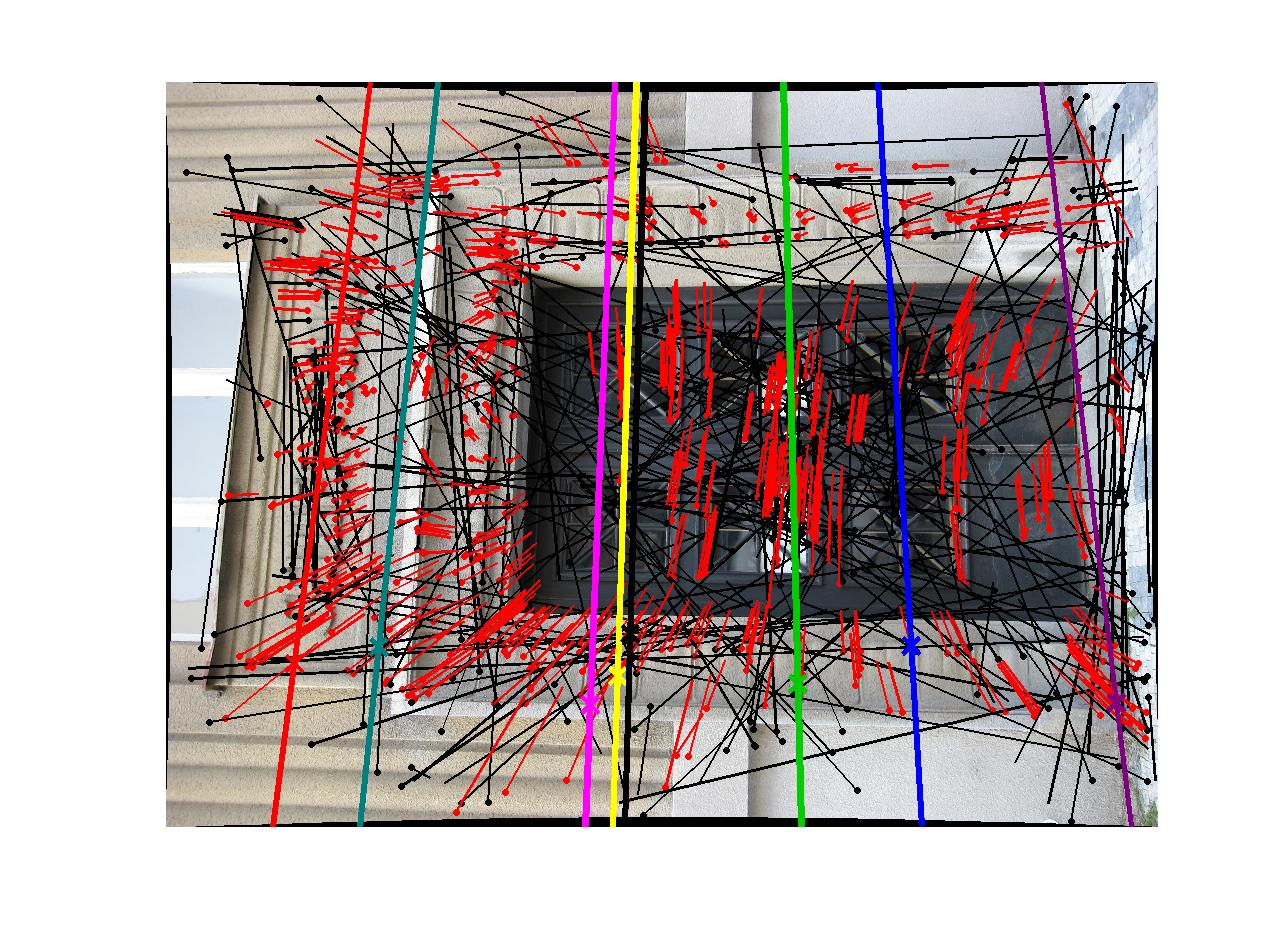
\includegraphics[width=9.3cm,angle=-90,clip=true,trim=165px 105px 110px 80px]{pictures/matches-left-with_epipolar_lines.jpg}}
			}
			\subfigure[] {
				\fbox{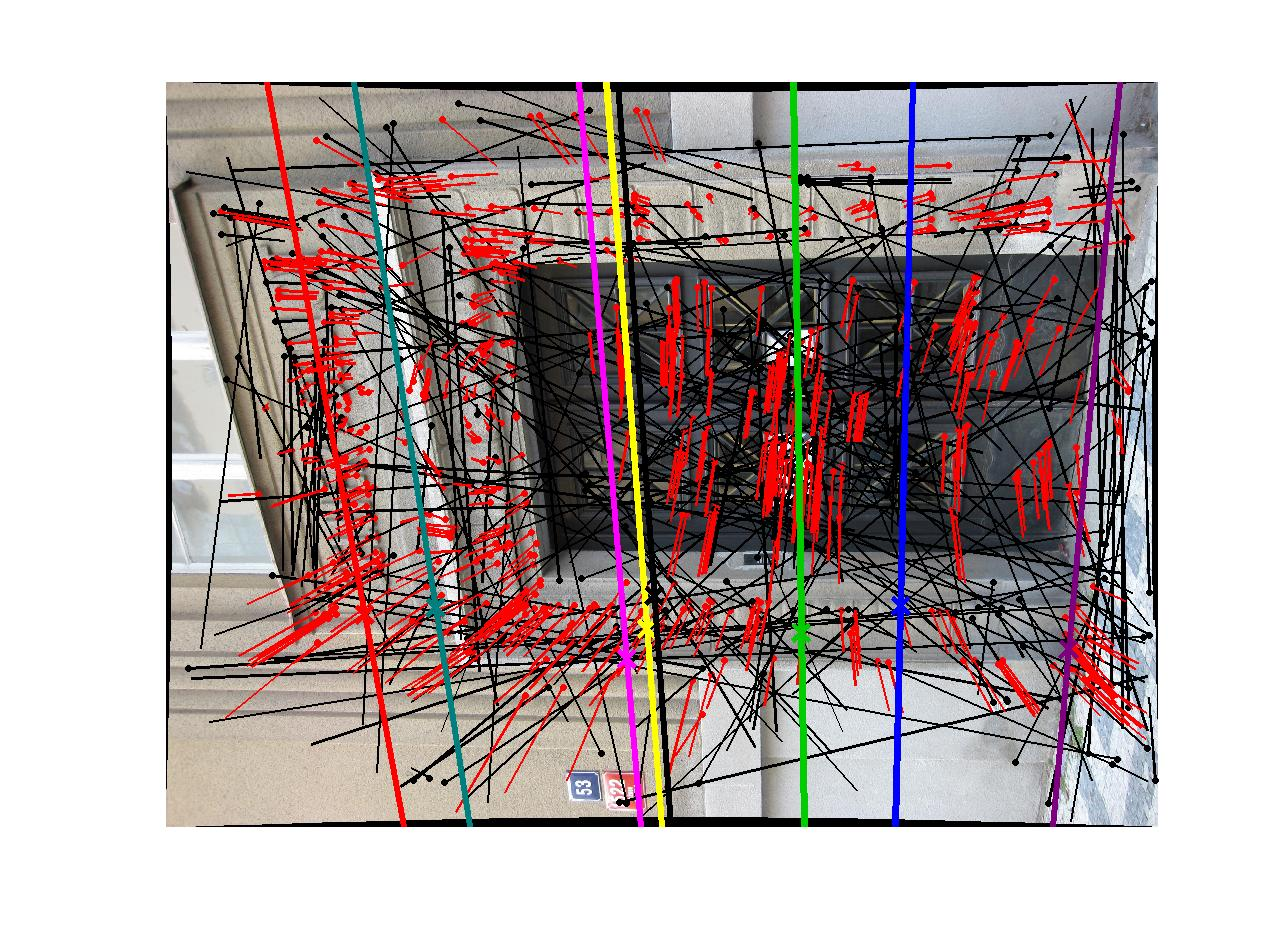
\includegraphics[width=9.3cm,angle=-90,clip=true,trim=165px 105px 110px 80px]{pictures/matches-right-with_epipolar_lines.jpg}}
			}
		\caption{Pár obrazů se zobrazenými korespondencemi: červeně korespondence odpovídající
			epipolární geometrii, černě chybné. Pro vybrané body (označené křížky) jsou
			stejnými barvami znázorněny vzájemně si odpovídající epipoláry. Obrazy
			odpovídají snímkům \ref{fig:i0} a \ref{fig:i1}. V obou obrazech je možné
			si všimnout podduškovitého obrysu okrajů, který vznikl po odstranění
			radiálního zkreslení.}
		\label{fig:korespondenceAEpipolary}
	\end{figure}

\paragraph{Hodnocení hypotéz} Každá nalezená dvojice kanonických kamer $\matrix P_1$, $\matrix P_2$ byla
testována oproti všem nalezeným korespondencím. Pro každou korespondenci byla spočtena reprojekční
chyba a byla určena opora hypotézy v datech jakožto počet korespondencí s reprojekční chybou menší
než empiricky určený práh (použili jsme práh odpovídající chybě 2 pixely v~každém obrazu).
Výsledkem RANSACu byla epipolární geometrie charakterizovaná rotací $\matrix R$ a translací $\matrix b$
a rozdělení korespondencí na inliery a outliery.

Pro vybraný pár obrazů jsou korespondence a epipoláry několika vybraných bodů zobrazeny na
\figref{fig:korespondenceAEpipolary}. Korespondence jsou znázorněny jako úsečky spojující
zvýrazněný bod z jednoho obrazu s místem, kde leží bod ve druhém obraze. Inliery jsou znázorněny
červeně, outliery černě. Počet použitých iterací v RANSACu (přesněji počet pětic korespondencí použitých
pro vytváření hypotéz) byl 38 pro jeden pár pohledů. Ve zobrazené dvojici pohledů jsou přibližně
70\% korespondencí inliery.


% - zkusit vypisovat úspěšnost RANSACu
% - vygenerovat data pro všechny páry
% - počet iterací RANSACu: 38
% - práh v RANSACu: 2px

% Notes:
%
% terminology:
%	correspondence = truth,
%	match = algorithm’s result; hypothesised corresp.

\dots

\section{Stereo}

Použili jsme \cite{Cech-BenCOS-CVPR-2007}


\section{Zhodnocení}

Na základě fotografií v \figref{fig:fotografie} a ze znalosti kalibrační matice kamery $\matrix K$
jsme určili vzájemnou geometrii párů kamer (jejich vzájemné otočení a směr posunutí). Dalším krokem
bude jejich umístění do společného souřadného systému.

V RANSACu jsme použili jednoduché prahování. Bylo by dobré porovnat kvalitu výsledků dosažených
s lepší robustní funkcí. Také by bylo vhodné dále optimalizovat esenciální matici nalezenou
RANSACem.

% FIXME: jak zahrnout bibliography.bib do repozitare? .. zkopirovat?

% Reference

	% FIXME:
	%	- zkontrolovat format oproti webu, zvolit vhodny .bst soubor
	%	- doplnit (?), aktualizovat odkazy a data

%\bibliographystyle{plain_cz}
\bibliographystyle{czechiso}
\bibliography{bibliography}

\end{document}

